%%%%%%%%%%%%%%%%%%%%%%%%%%%%%%%%%
% CMPSC 280
% Authors: Michael Camara, Colton McCurdy, Jake Hanko, Keegan Shudy, Victor Zheng, Cody Kinneer
% Honor Code Pledge: This work is ours unless otherwise cited
% Purpose: Presentation slides for Repo-Rover on 10/2/15
%%%%%%%%%%%%%%%%%%%%%%%%%%%%%%%%%

\documentclass{beamer}
\usepackage{graphicx}
\usetheme{Frankfurt}
\setbeamertemplate{blocks}[rounded]
\setbeamercolor{structure}{fg=red}
\usepackage{multicol}

\usepackage{tikz-er2}  % Entity-Relation Diagram Package
% Author: Pável Calado
% the tikz-er2.sty package is available at:
% http://tagus.inesc-id.pt/~pcalado/tikzer2/tikz-er2.html

% Packages for use with tikz-er2 / drawing
\usepackage{verbatim}
\usetikzlibrary{positioning} 
\usetikzlibrary{shadows}
\usepackage{tikz}
\tikzstyle{line}=[draw]
\tikzstyle{arrow}=[draw, -latex] 
\setbeamertemplate{headline}[default] % remove dark edge on top

%% Styles for diagram nodes
\tikzstyle{every entity} = [top color=white, bottom color=blue!30,
draw=blue!50!black!100, drop shadow]
\tikzstyle{every weak entity} = [drop shadow={shadow xshift=.7ex,
shadow yshift=-.7ex}]
\tikzstyle{every attribute} = [top color=white, bottom color=yellow!20,
draw=yellow, node distance=1cm, drop shadow]
\tikzstyle{every relationship} = [top color=white, bottom color=red!20,
draw=red!50!black!100, drop shadow]
\tikzstyle{every isa} = [top color=white, bottom color=green!20,
draw=green!50!black!100, drop shadow]

%% Create background of Mars landscape with a rover and some Git repos
\usebackgroundtemplate{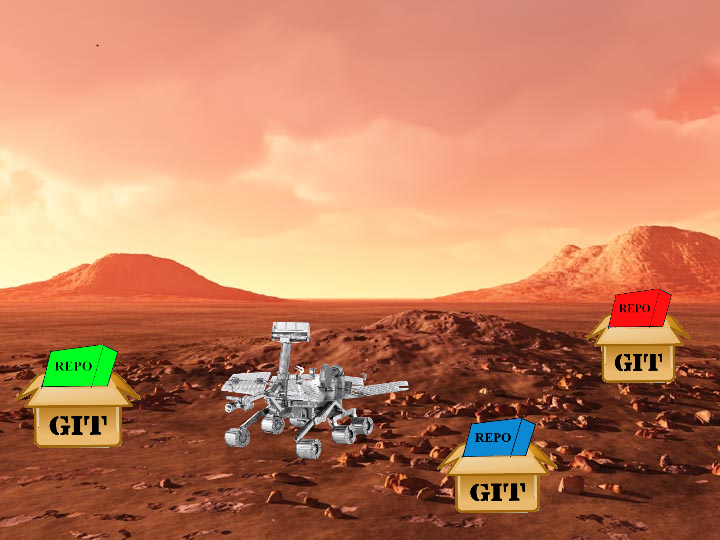
\includegraphics[width=\paperwidth]{images/landscape.png}}

\begin{document}

%% TITLE PAGE
\begin{frame}
    \centering
    \vspace{-1in}
    \emph{\textcolor{black}{\textbf{
    	\Huge “Repo-Rover”\\
    \begin{multicols}{2}
    	\large Colton McCurdy\\Jake Hanko\\Michael Camara\\
	\columnbreak
		\large Keegan Shudy\\Victor Zheng\\Cody Kinneer\\
	\end{multicols}
    }}}
\end{frame}

%% Create white overlay over background to enhance clarity of text
\usebackgroundtemplate{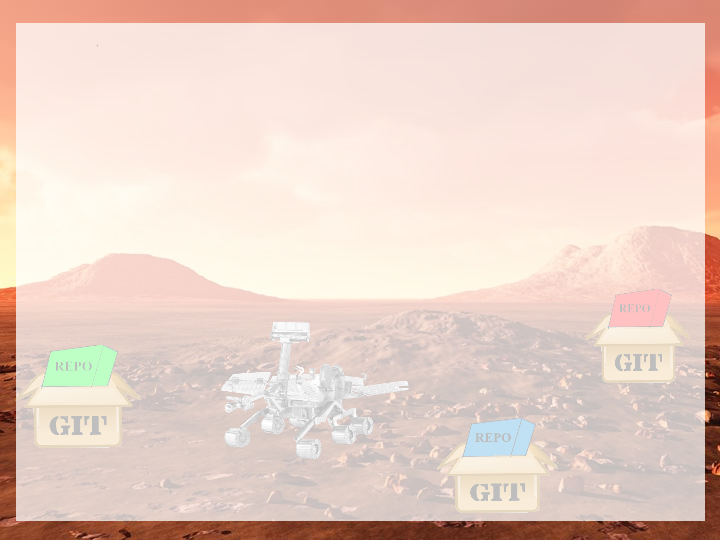
\includegraphics[width=\paperwidth]{images/landscape_white_overlay.png}}

%% INTRODUCTION
\begin{frame}
    \centering
    \frametitle{Git}
    
    \begin{block}{What is Git?}
		Git is version control system that "records changes to a file or set of files over time so that you can recall specific versions later."\textsuperscript{1}
    \end{block}

    \resizebox{11cm}{5cm}{
	    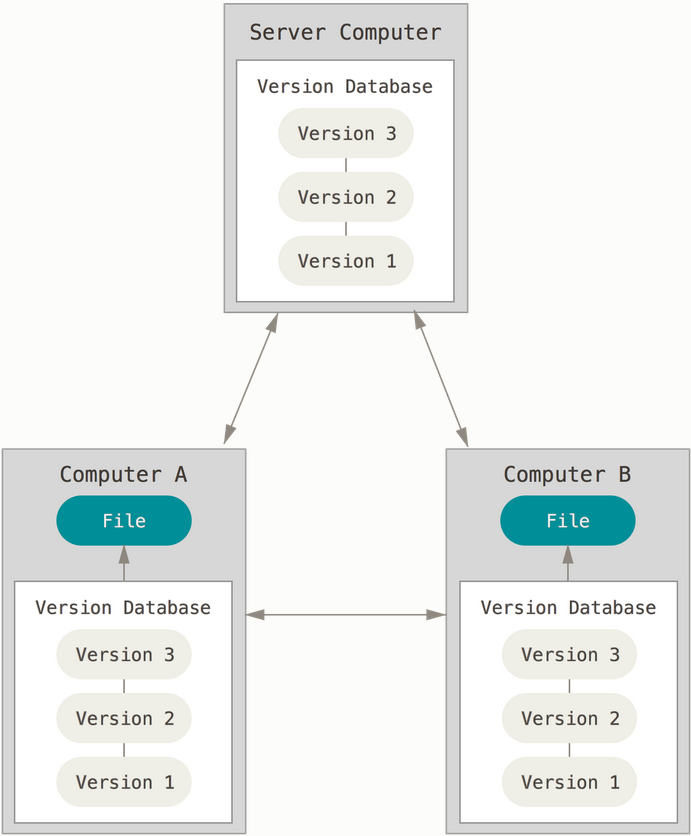
\includegraphics{images/git_diagram1.png}
	} % end resizebox 
\end{frame}
     
\begin{frame}

    \centering
    \frametitle{The Repo Problem}

	\begin{block}{Git gaining in popularity}
		\begin{itemize}
			\item GitHub: 27.3 million repositories, 11 million users\textsuperscript{2}
			\item Bitbucket: 2.5 million users\textsuperscript{3}
			\item 1 in 3 Fortune 500 companies use Git for 60\% of their source code\textsuperscript{4}
		\end{itemize}
	\end{block}    
	
	\pause 
	
    \begin{block}{So many repos, so little time...}
    		Computer scientists need a better way to maintain all of their Git repos!      
    \end{block}
    
    \resizebox{11cm}{3.0cm}{
	    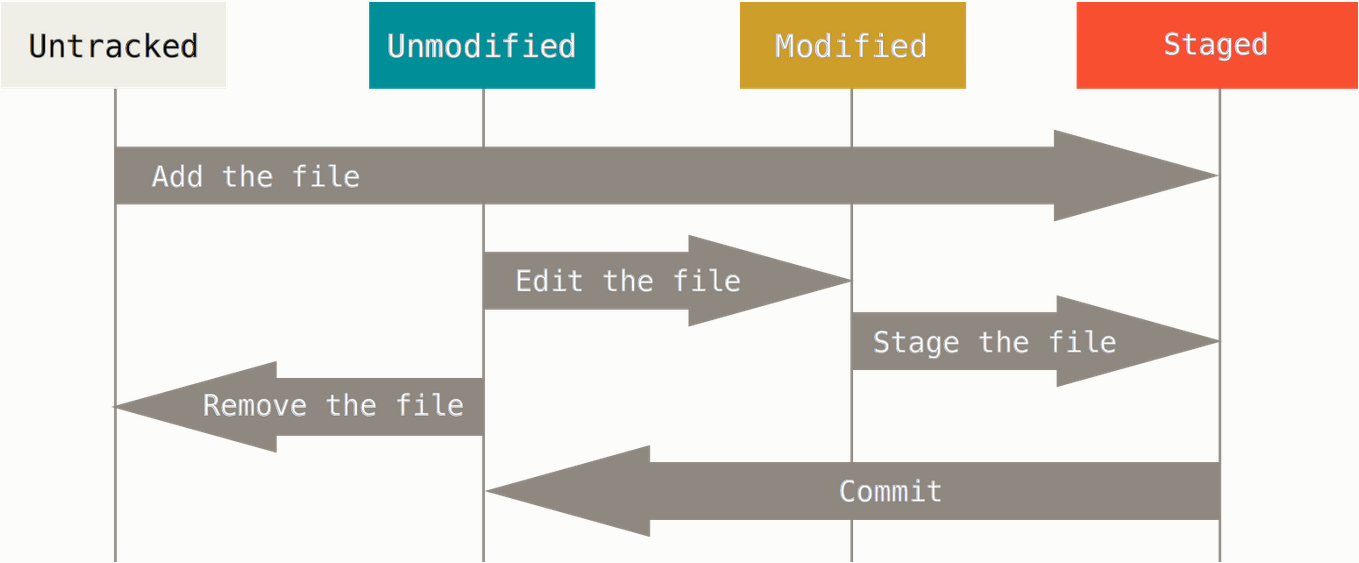
\includegraphics{images/git_diagram2.png}
	} % end resizebox 
    	
\end{frame}

\begin{frame}{animate}
	\centering
	\frametitle{Existing Solutions}
	
	\begin{block}{Git Commands}
		\begin{itemize}
			\item git status
			\item git log
		\end{itemize}
	\end{block}
	
	\pause
	
	\begin{block}{External Programs}
		\begin{itemize}
			\item Gitinspector: https://github.com/ejwa/gitinspector
			\item GitStats: http://gitstats.sourceforge.net/
		\end{itemize}
	\end{block}
		%\animategraphics[controls,autoplay,loop,width=4cm,poster=first]{1}{images/cats}{0}{61}
	
	\pause	
	
    \resizebox{11cm}{4.2cm}{
	    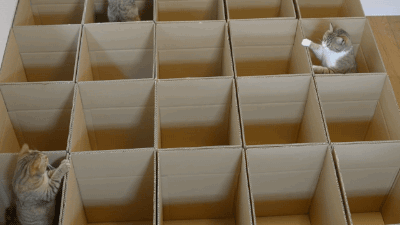
\includegraphics{images/cats.png}
	} % end resizebox 
	
	\

\end{frame}

%% Add related works??

% Requirements 1/  :Summary
\begin{frame}
	\centering
	\frametitle{Requirements}
	\begin{block}{Summary}
		Repo-Rover must traverse a user's filesystem from given a root address, locate all Git repos contained therein, and provide relevant diagnostic information to the user.
	\end{block}
	
	\resizebox{11cm}{2.5cm}{%
	\begin{tikzpicture} [node distance = 7em]
		\node[entity] (system) {Filesystem};
		\node[relationship] (contains) [right of=system, node distance = 10 em] {Contains} edge node[auto, swap] {1} (system);		
		
		% Middle branch
		\node[entity] (repo) [right of=contains, node distance = 10 em] {Git Repo} edge[total] node[auto, swap] {n} (contains);

		\node[attribute] (mid_feature1) [above right of=repo, node distance = 5 em] {\discriminator{Feature 1}} edge (repo);
		\node[attribute] (mid_feature2) [right of=repo, node distance = 7 em] {\discriminator{Feature 2}} edge (repo);
		\node[attribute] (mid_feature3) [below right of=repo, node distance = 5 em] {\discriminator{Feature 3}} edge (repo);
	\end{tikzpicture}
	}
	
		\pause
	\begin{block}{Purpose}
			To provide an easy, automated means for computer scientists to monitor their Git repositories and avoid potentially costly oversights.
	\end{block}
\end{frame}

% Requirements 2/  :Constraints
\begin{frame}
	\centering
	\frametitle{Requirements}
	\begin{block}{Process Constraints}
		\begin{enumerate}
			\item Incremental Development
			\item Documentation
			\item Public Access
		\end{enumerate}
	\end{block}
	\pause
	\begin{block}{Design Constraints}
		\begin{enumerate}
			\item Audience
			\item Programming Language
			\item Operating System
			\item Interface (Input/Output)
		\end{enumerate}
	\end{block}
\end{frame}

% Requirements 3 /
\begin{frame}
	\centering
	\frametitle{Requirements}
	\begin{block}{Functional Requirements}
		\begin{enumerate}
			\item <1-> Filesystem traversal
			\item <2->Diagnostic Summary (\textbf{Per} Repo)
			\pause
			\begin{itemize}
				\item <3-> Files with untracked modifications
				\item <3-> Files in staging area
				\item <3-> Committed files not pushed
			\end{itemize}
			\item <4-> Diagnostic Summary (\textbf{All} Repos)
			\begin{itemize}
				\item <5-> Total number of repos
				\item <5-> Percentage of "clean" repos
			\end{itemize}
		\end{enumerate}		
	\end{block}
\end{frame}
\tikzstyle{class} = [ellipse, minimum width=4.5cm, minimum height=1cm,text centered, draw=black, fill=yellow!30]
\tikzstyle{input} = [trapezium, trapezium left angle=70, trapezium right angle=110, minimum width=5cm, minimum height=2cm, text centered, draw=black, fill=blue!30]
\tikzstyle{output} = [trapezium, trapezium left angle=70, trapezium right angle=110, minimum width=5cm, minimum height=2cm, text centered, draw=black, fill=green!30]
\tikzstyle{method} = [rectangle, minimum width=5cm, minimum height=2cm, text centered, draw=black, fill=orange!30]
\tikzstyle{base} = [rectangle, rounded corners, minimum width=2cm, minimum height=2cm,text centered, draw=black, fill=red!30]
\tikzstyle{cond} = [diamond, minimum width=5cm, minimum height=2cm, text centered, draw=black, fill=white!30]
\tikzstyle{arrow} = [thick,->,>=stealth]

% Design Template
\begin{frame}
	\centering
	\frametitle{Design}

	\begin{block}{Programming Language: Python}
	We chose to use Python because...
		\begin{enumerate}
			\item 
			\item 
		\end{enumerate}	
	\end{block}
	
	\pause
	
	\begin{block}{Input}
	\end{block}
	
	\pause
	
	\begin{block}{Output}
	\end{block}
	
\end{frame}

\begin{frame}
	\centering
	\frametitle{Design}
	\begin{block}{Program Structure}
		\begin{enumerate}
			\item 
%			\item find\_git\_report
%			\item git\_issues
%			\item write\_reports
%			\item has\_issues
%			\item get\_file
%			\item get\_file\_new
%			\item get\_unpushed
%			\item get\_commits\_behind
%			\item write\_report
		\end{enumerate}	
	\end{block}	
\end{frame}


%Design Diagram
% NEED TO UPDATE WITH NEW DESIGN DIAGRAM
\begin{frame}
	\centering
	\frametitle{Design}
	
	% Adjust dimensions of resize box as desired
	\resizebox{7cm}{7.5cm}{
	
		\begin{tikzpicture}[node distance=2cm]

% objects
\node (class) at (0,0) [class] {\texttt{Path of the Directory}};
\node (method1) at (0,-3) [method] {\texttt{find\_git\_repos(Directory)}};

\node (method2) at (0,-6) [method] {\texttt{git\_issues(Directory)}};

\node (method3) at (0,-9) [method] {\texttt{has\_issues()}};
\node (method4) at (0,-13) [method] {\texttt{write\_report()}};


% \node (method4) at (8,-13) [method] {\texttt{incPos(temp, pos, size)}};
\node (base) at (0,-16) [base] {\texttt{html report}};


% arrows
%\draw [arrow] (class) -- (method1);
\draw [arrow] (class) -- node[anchor=east] {user-input} (method1);
\draw [arrow] (method1) -- (method2);
\draw [arrow] (method2) -- (method3);
\draw [arrow] (method3) -- node[anchor=east] {return issue\_list} (method4);
\draw [arrow] (method4) -- (base);

		\end{tikzpicture}	
	} %end resizebox

\end{frame}
% Implementation Template
\begin{frame}
	\centering
	\frametitle{Begin the Demonstration!}
	
	\resizebox{11cm}{4cm}{
	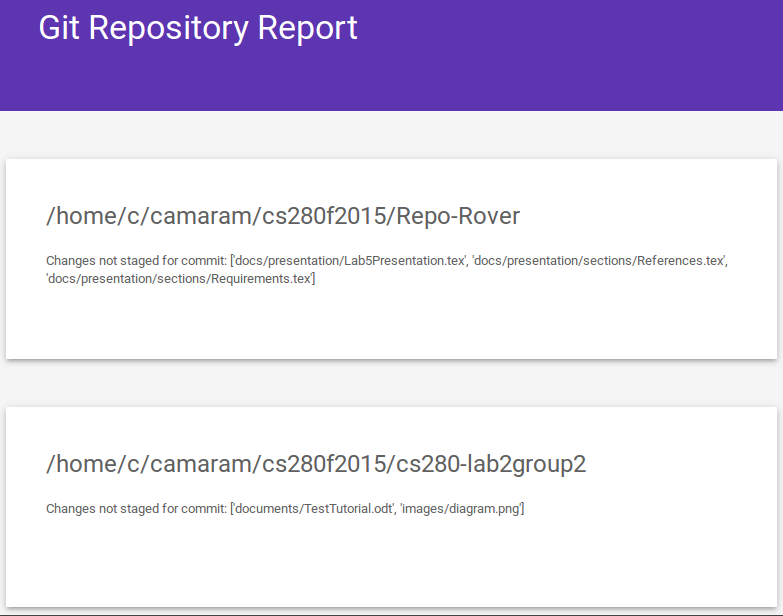
\includegraphics[]{images/output_html.png}	
	}	
	
	\vspace{0.25cm}

	\resizebox{11cm}{4cm}{
	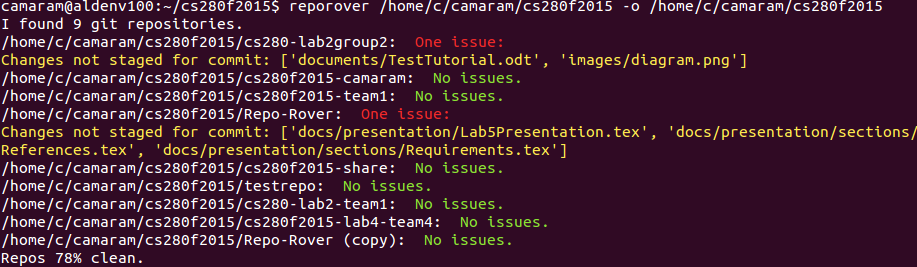
\includegraphics[]{images/output_console.png}	
	}


	
\end{frame}

% Testing template
\begin{frame}
	\centering
	\frametitle{Testing}

	\begin{block}{Testing Strategy}
		
	 Comparing the number of expected repositories with actual repositories (Unit testing to verify the correctness of our system )
			\begin{center}
			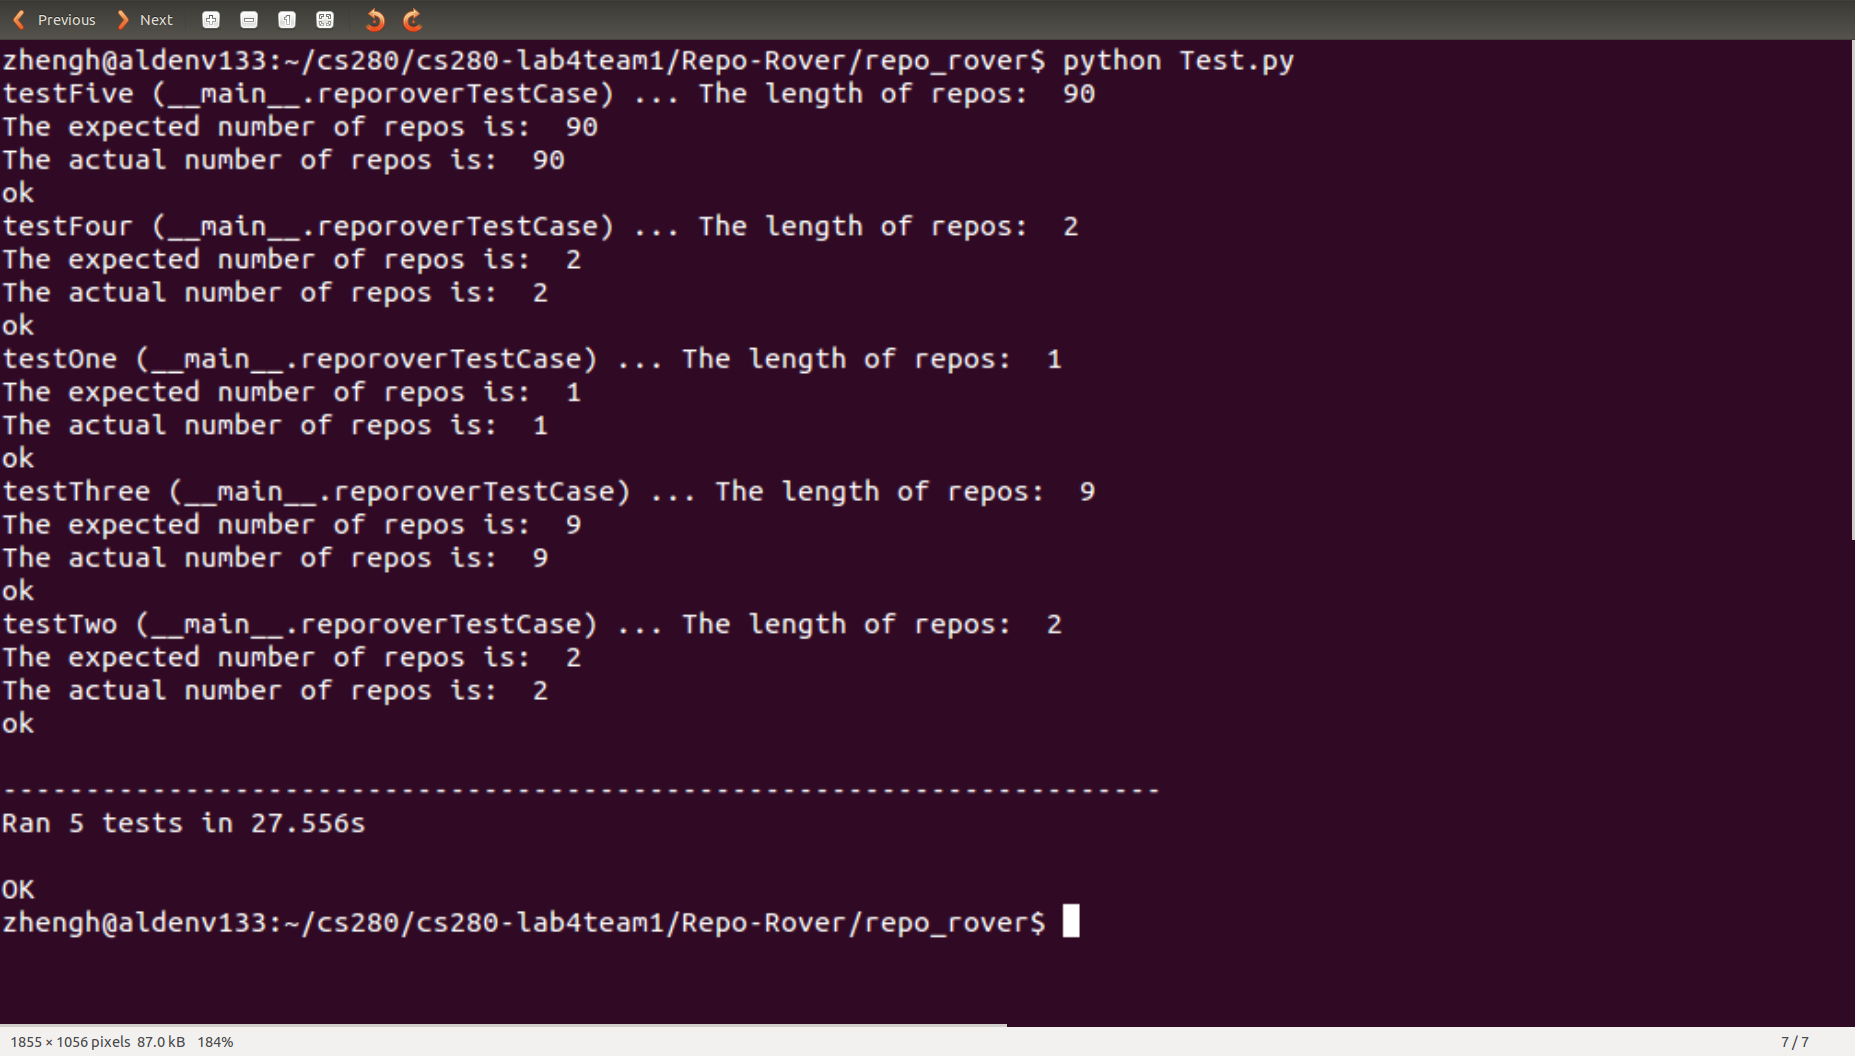
\includegraphics[width=10cm, height=5cm]{images/TestingResult.png}
			\end{center}
		
	\end{block}
	
\end{frame}

\begin{frame}
	\begin{block}{System Performance}
	The execution time of running the program with different repositories: 
		\begin{center}
			\begin{table}[]
			\centering
			\begin{tabular}{lll}
			\hline
 			1 Repository& 9 Repositories & 90 Repositories \\
 			0.217&1.285  &27.367    \\
 			\hline
 			0.218&1.275  &28.191    \\
 			\hline
 			0.203&1.281  &27.689		\\
 			\hline   
 			0.206& 1.279 & 27.514	\\
 			\hline
 			0.202& 1.283	 & 27.212	\\
 			\hline
 			Mean Value: & Mean Value: & Mean Value: \\
 			0.2092 & 1.2806	& 27.5946 
			\end{tabular}
			\end{table}
		\end{center}		
	\end{block}	
\end{frame}

\begin{frame}
	\begin{block}{System Performance}
	\begin{center}
	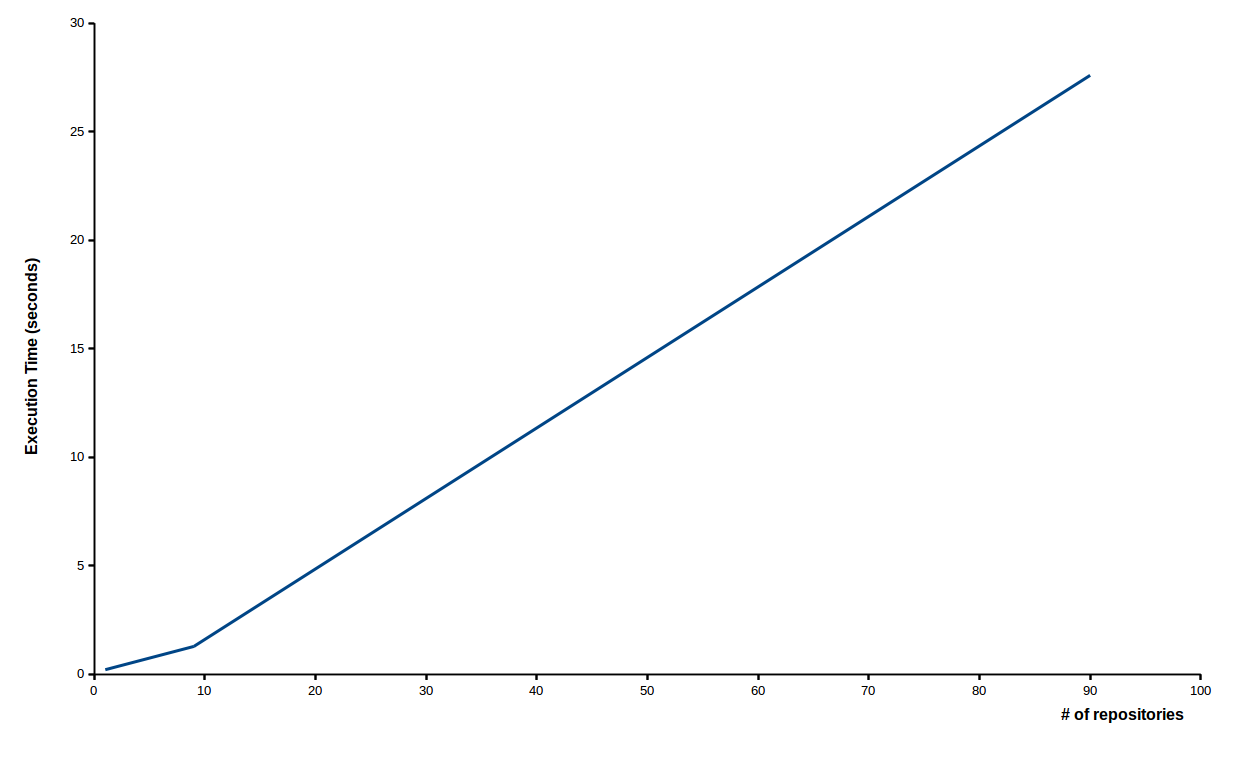
\includegraphics[width=10cm, height=7cm]{images/Execution.png}
	\end{center}
	\end{block}	
\end{frame}

% Release template
\begin{frame}
	\centering
	\frametitle{Release}

	\begin{block}{Issues Reported and Resolved}
		\begin{enumerate}
			\item Cloning
			\item CSS
			\item README
		\end{enumerate}
	\end{block}

	\pause

	\begin{block}{Unresolved Issues}
		\begin{enumerate}
			\item Windows
		\end{enumerate}
	\end{block}

	\pause

	\begin{block}{Challenges}
		\begin{enumerate}
      \item Operating System (Windows)
			\item Executable Shell Command
			\item SSH v. HTTPS
		\end{enumerate}
	\end{block}

\end{frame}


%% FUTURE WORK
%TODO need to revise and add onto this
\begin{frame}
    \centering
    \frametitle{Future Work}
    
    \begin{block}{Ideas for Improvement}
    		\begin{enumerate}
    			\item Implement a GUI
    			\item Allow "garbage file" recognition
    			\item Add Windows support
    		\end{enumerate}
    \end{block}
    
\end{frame}

%% CONCLUSION
%TODO consider adding block in here
\begin{frame}
    \centering
    \frametitle{Conclusion}
    \begin{block}{}
    \begin{center}
	\emph{\huge{\textbf{Your years of clutter are over: get yourself a Repo-Rover!}}}
    \end{center}
    \end{block}
	\vspace{3.5cm}
    \begin{block}{}
    \begin{center}
    \emph{\Large{Available Now At \emph{https://github.com/keggster101020/Repo-Rover}}}
    \end{center}
    \end{block}
\end{frame}

%% References
\begin{frame}
    \centering
    \frametitle{References}
	\fontsize{9}{7.2}
	\begin{enumerate}
		\item Chacon, S. \& Straub, B.  (2014).  Pro Git.  https://git-scm.com/book/en/v2/Getting-Started-About-Version-Control
		\item GitHub Press Release.  (2015).  Retrieved from https://github.com/about/press
		\item Sarkar, R.  (2015).  "Bitbucket: 2014 in review."  Retrieved from https://blog.bitbucket.org/2015/02/05/bitbucket-2014-in-review/
		\item Sarkar, R.  (2015).  "1 in 3 Fortune 500 companies agree: Bitbucket is the Git solution for professional teams."  Retrieved from http://blog.bitbucket.org/2015/09/22/1-in-3-fortune-500-companies-agree-bitbucket-is-the-git-solution-for-professional-teams/
	\end{enumerate}	

	\vspace{1.5cm}	
	
	\begin{block}{}
    \begin{center}
    \emph{\Large{Available Now At \emph{https://github.com/keggster101020/Repo-Rover}}}
    \end{center}
    \end{block}
    
\end{frame}

\begin{frame}
    \centering
    \frametitle{References}
	\fontsize{9}{7.2}
	Images:
	\begin{itemize}
		\item Mars Rover: http://eugenetoyandhobby.com/shop/metal-earth-mars-rover/
		\item Mars Landscape: http://bytescapes.com/natural/one-step-beyond/martian-landscape/
		\item Git Box: http://www.layeredthoughts.com/git/private-remote-git-repositories-ubuntu-linode
		\item Git Diagrams: http://git-scm.com/book/en/v2/Getting-Started-Git-Basics
		\item Gears: http://www.industryqualifications.org.uk/sectors/functionalskills
		\item Thumbs-Up:  https://bpaquality.wordpress.com/2014/01/30/common-sense-quality/
		\item Constraints: http://www.halogensoftware.com/blog/how-to-master-employee-engagement-constraints
		\item Cats: http://rottenpanda.com/cat-heaven/
	\end{itemize}
	\begin{block}{}
    \begin{center}
    \emph{\Large{Available Now At \emph{https://github.com/keggster101020/Repo-Rover}}}
    \end{center}
    \end{block}
\end{frame}

\end{document} 


